\documentclass[12pt,a4paper]{article}
\usepackage[utf8]{inputenc}
\usepackage[OT1]{fontenc}
\usepackage{amsmath}
\usepackage{amsfonts}
\usepackage{amssymb}
\usepackage{graphicx}
\usepackage{tikz}
\usepackage{pgfplotstable}
\usepackage{mathtext}

\usepackage[T1]{fontenc}
\usepackage[utf8]{inputenc}
\usepackage[english, bulgarian, russian]{babel}

\usepackage{tikz}
\usepackage{pgfplots}
\usepackage{indentfirst}
\usepackage[export]{adjustbox}
\usepackage{multirow}
\usepackage{geometry} \geometry{verbose,a4paper,tmargin=2cm,bmargin=2cm,lmargin=1.5cm,rmargin=1.5cm}

\graphicspath{{Images/}}
\usepackage[left=2cm,right=2cm,top=2cm,bottom=2cm]{geometry}
\usepackage{wrapfig}
\usepackage{setspace}
\usepackage{indentfirst}
\usepackage{subfigure}


\begin{document}

\begin{titlepage}
  \begin{center}
    \huge
    Московский Физико-технический Институт
    
    (Национальный исследовательский университет)
    \vspace{0.5cm}

   
    \vspace{0.25cm}
 
    \vfill
 
    \vfill

    \textsc{\bf{Отчет о выполнении работы 2.2.3}}\\[3mm]
    
    {\LARGE  Измерение теплопроводности воздуха при атмосферном давлении}
  \bigskip
    \vfill
    
\end{center}
\vfill
\begin{flushright}

    Выполнили студентки 1 курса
    
    ФБМФ, группа Б06-103

    Попеску Полина
    
    
    Фитэль Алёна

\end{flushright}
\bigskip


\vfill

\begin{center}
  Долгопрудный, 2022 г.
\end{center}
\end{titlepage}

\section{Введение}

\textbf{Цель работы:} измерить коэффициент теплопроводности воздуха при атмосферном
давлении в зависимости от температуры.


\textbf{В работе используются:} цилиндрическая колба с натянутой по оси нитью; термостат;
вольтметр и амперметр (цифровые мультиметры); эталонное сопротивление; источник
постоянного напряжения; реостат (или магазин сопротивлений).

\section{Теоретический материал}
Основной характеристикой теплопроводности служит коэффициент $\varkappa$, являющийся коэффициентом пропорциональности между плотностью потока тепла $q$ и градиентом температуры $dT/dr$ в направлении распространения этого потока
\begin{equation}
	q = -k \frac{dT}{dr}.
\end{equation}

	В цилиндрически симметричной установке, в которой тепловой поток направлен к стенкам цилиндра от нити, полынй поток тепла $Q = qS$ через каждую цилиндрическую поверхность радиуса $r$ должен в стационарном состоянии быть неизменен (как в пространстве, так и во времени). Тогда
\begin{equation}
	Q = -2\pi rLk \frac{dT}{dr} = const,	
\end{equation}
Если перепад температуры $ \Delta T =T_2-T_1$ между нитью и стенками цилиндра мал ($ \Delta T\ll T_1 $) в (2) можно пренебречь изменением теплопроводности от температуры в пределах системы, положив $k\approx k(T_1)$. Тогда разделяя переменные в (2) и интегрируя от радиуса нити до радиуса колбы, получим
\begin{equation}
Q=\frac{2\pi L}{\ln(\frac{r_1}{r_2})}k\cdot\Delta T
\end{equation}
откуда получаем формулы:
\begin{equation}
	\label{formula}
	T_1 - T_2 = \frac{Q}{2\pi Lk} \ln \frac{r_2}{r_1}.
\end{equation}
\begin{equation}
	\label{formula}
	k= \frac{Q\cdot \ln \frac{r_2}{r_1}}{2\pi L\cdot\Delta T}.
\end{equation}
Здесь $r_1$ и $T_1$ -- радиус и температура нити, $r_2$ и $T_2$ -- радиус и температура цилиндра.

 \section{Экспериментальная установка}
 Схема лабораторной установке представлена на рисунке 1. Тонкая молибденовая проволока натянута по оси вертикально стоящей медной трубки. Через штуцер трубка заполняется исследуемым газом. Нить нагревается электрическим током, ее температура $T_1$ определяется по изменению электрического сопротивления. Трубка находится в кожухе, через который пропускается вода из термостата. Температура воды $T_2$ измеряется термометром, помещенным в термостат. Количество теплоты,
протекающей через газ, равно (если пренебречь утечками тепла через торцы) количеству теплоты, выделяемому током в нити, и может быть найдено по закону Джоуля—Ленца. При этом ток в нити определяется по напряжению на включенном последовательно с ней эталонном сопротивлении 10 Ом. Таким образом, все величины, входящие в правую часть формулы (1), поддаются непосредственному измерению. \par
\newpage
\begin{figure}[h!]
    \centering
    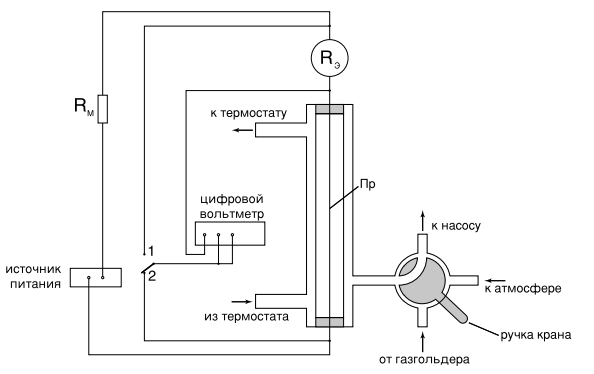
\includegraphics[width=12 cm]{setup.png}
    \caption{Схема установки для определения теплопроводности газов}
    \label{fig:vac}
\end{figure}

Электрическая часть схемы состоит из источника питания и под-
ключенных к нему последовательно соединенных нити, эталонного
сопротивления 10 Ом и магазина сопротивлений $R_M$, служащего для
точной установки тока через нить. Цифровой вольтметр может подключаться как к нити, так и к эталонному сопротивлению, измеряя
таким образом напряжение на нити и ток через нее.

\begin{figure}[h!]
    \centering
    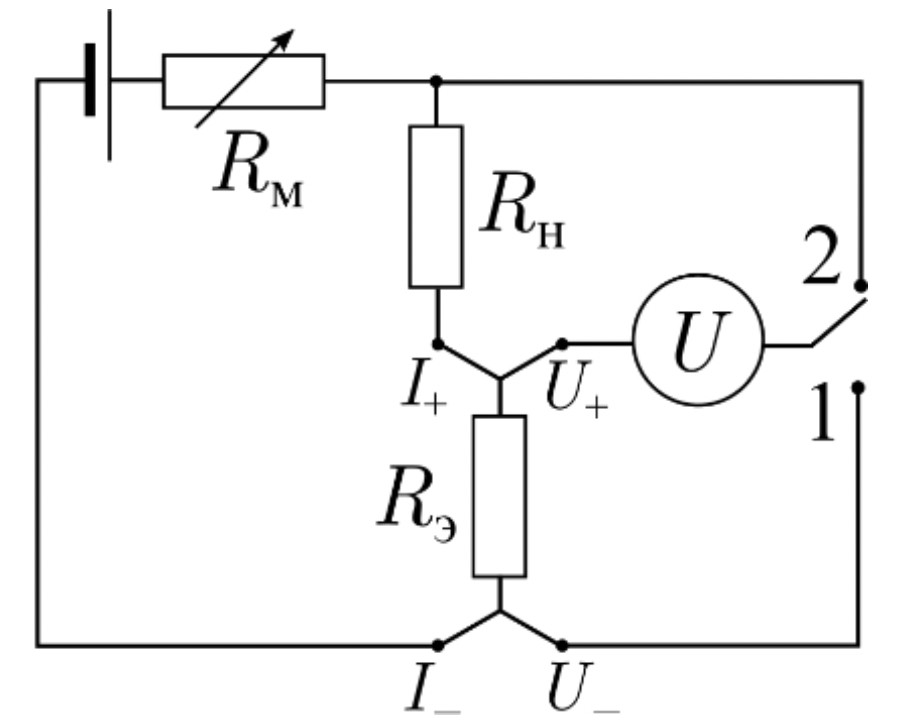
\includegraphics[width=7 cm]{electr.png}
    \caption{Электрическая часть схемы установки}
    \label{fig:elect}
\end{figure}

Сопротивление нити может быть измерено по формуле:
\begin{equation}
	\label{eq:rniti}
	R_H = R_0 \frac{U_H}{U_0}
\end{equation}

Выделяемая мощность рассчитывается по формуле:
\begin{equation}
	\label{eq:q_eq}
Q = \frac{U_H U_0}{R_0}
\end{equation}


Параметры установки:
$L = 347$ мм; $2r_1 = 0,050 \pm 0,005$ мм, $2r_2 = 10,0 \pm 0,1$ мм $ln(r_2/r_1) = 5,30, R_0 = 10,000 \pm 0,001$ Ом, $R_н = 17,5$ Ом.

\section{Обработка результатов измерений}

\begin{enumerate}
 \item Проведем предварительные расчеты параметров опыта. Приняв максимальный перегрев нити относительно термостата равным $ \Delta T_{max}=10^\circС$, оценим максимальную мощность нагрева $Q_{max}$, которую следует подавать на нить, а с ее помощью найдем максимальный ток и напряжение, которые можно подавать системе. Для этого используем уравнение (4), и закон Ома, из которого:
 \begin{center}
 $I_{max}=\sqrt{\frac{Q_{max}}{R}}$ \hspace{70}
 $U_{max}=\sqrt{Q_{max}R}$
\end{center}
Для этой оценки используем значение коэффициента теплопроводности воздуха $k\approx25\frac{\text{мВт}}{\text{м}\cdot\text{К}}$ и приближенное значение сопротивления нити $R_н$, указанное на установке, из которых получим:
\begin{center}
 $Q_{max}=0,10\text{Вт}$\hspace{40}
 $I_{max}=0,07\text{A}$\hspace{40}
 $U_{max}=1,3\text{В}$
\end{center}


  \item При температурах от 22 до 70$^\circ$C измерим зависимость сопротивления нити $R_н$ от подаваемой на нее мощности $Q$, не превышающей $Q_{max}$. Сопротивление нити рассчитывается по формуле (\ref{eq:rniti}). Выделяемая мощность рассчитывается по формуле (\ref{eq:q_eq}). Для каждой температуры термостата построим график зависимости сопротивления нити от мощности $R(Q)$.
    \begin{figure}[h!]
    \centering
    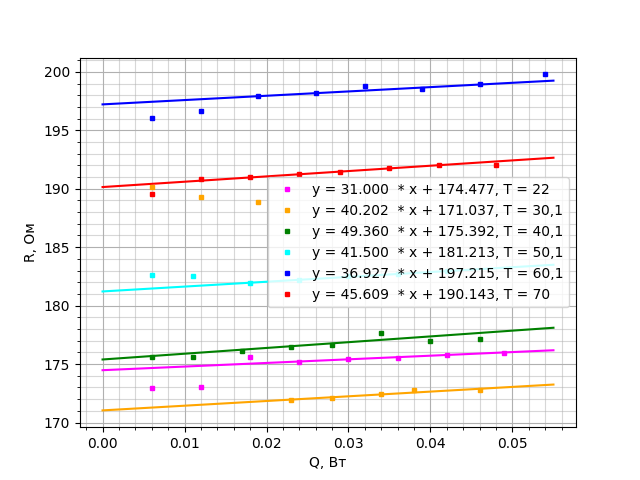
\includegraphics[scale=0.72]{R(Q).png}
    \caption{Зависимость R(Q)}
\end{figure}
     Из них получим:
     \begin{table}[!h]
	\centering
	\begin{tabular}{|1|1|1|}
		\hline
		Температура термостата,$^\circ$C     & $\frac{\text{d}R}{\text{d}Q}\frac{\text{Ом}}{\text{Вт}}$  & $R_0$, Ом\\ \hline
		22,0 & 31\pm 3 & 174,48\pm 0,02 \\ \hline
		30,1 & 40\pm 6 & 171,04\pm 0,05 \\ \hline
		40,1 & 50\pm 16 & 175,39\pm 0,14 \\ \hline
		50,1 & 41\pm 2 & 181,21\pm 0,02 \\ \hline
		60,1 & 37\pm 2 & 197,21\pm 0,03 \\ \hline
		70,0 & 45\pm 1 & 190,14\pm 0,01 \\ \hline
	\end{tabular}
		\caption{Данные, полученные из графика на рис. 3}
\end{table}
 \item Используя полученные из графиков методом экстраполяции значения $R_0$, построим график зависимости сопротивления нити от температуры $R(T)$. Из него получим значение углового коэфициента наклона прямой $\frac{\text{dR}}{\text{d}T}=0,48\pm0,12~ \frac{\text{Ом}}{C^\circ }$ и значение $R_{273}=160\pm2~ \text{Ом}$ ($R_{273}$ - сопротивление нити при $273 K$). С помощью этих данных определим температурный коэффициент сопротивления материала нити: $\alpha=\frac{1}{R_{273}}\cdot\frac{\text{dR}}{\text{d}T}$, получим $\alpha=(3,0\pm0,8) \cdot 10^{-3}~\frac{1}{C^\circ} $.
 \begin{figure}[h!]
    \centering
    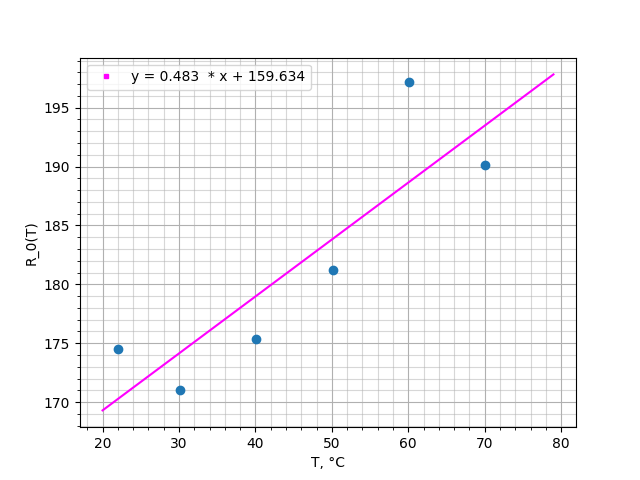
\includegraphics[scale=0.72]{R_0_T.png}
    \caption{Зависимость $R_0$(T)}
\end{figure}
\item Используя угловой коэффициент температурной зависимости сопротивления $\frac{\text{dR}}{\text{d}T}$ из п.3 и угловые коэффициенты нагрузочных прямых $\frac{\text{dR}}{\text{d}Q}$ из п.2, найдем коэффициенты теплопроводности газа $k$ для каждой температуры термостата $T_1$, используя формулу (5), в которой зависимость выделяющейся на нити мощности от ее перегрева относительно стенок расчитаем с помощью полученных раннее значений: $\frac{\text{dQ}}{\text{d}T}$=$\frac{\text{dR}}{\text{d}T} / \frac{\text{d}R}{\text{d}Q}$. Для полученных значений построим график зависимости $k(T)$:

\item Предполагая, что $k$ степенным образом зависит от температуры: $k\sim T^{\beta}$, построим график в двойном логарифмическом масштабе и определим из него показатель степени $\beta$, равный коэффициенту наклона прямой. Погрешности значений $k$ сильно отличаются друг от друга, поэтому для нахождения коэффициентов прямой воспользуемся методом взвешенного МНК.

Так, получим $\beta=0,40\pm0,05$.
\begin{figure}[h!]
    \centering
    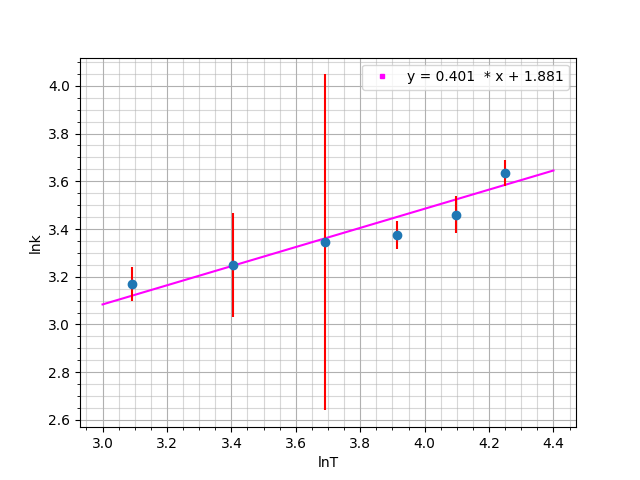
\includegraphics[scale=0.72]{lnk(lnT).png}
    \caption{Зависимость $lnk(lnT)$}
\end{figure}


\end{enumerate}
\newpage

\section{Вывод}

1. В ходе проведенной работы были определены коэффициенты теплопроводности воздуха при атмосферном давлении в зависимости от температуры по теплоотдаче нагреваемой током нити в цилиндрическом сосуде. Для этого были измеренны зависимости значений сопротивления нити от подаваемой на нее мощности, которые в условиях данного опыта должны быть линейными, в силу выбранного рабочего диапазона температур. Из-за
существенного вклада термоэлектрических явлений в проводниках и контактах точность измерений при малых токах невелика. Чем меньший ток мы пропускаем, тем с меньшей точностью у нас измеряется сам ток и напряжение. Вследствие этого первые три точки существенно отклоняются от остальных (см. прямые 2, 4, 5, 6). На прямой 2 при учете первых трех точек получается отрицательный наклон прямой, а следовательно, отрицательная теплопроводность, что говорит о явной ошибке в измерениях. Поэтому при подсчете коэффициентов прямых мы не учитывали первые три точки. 

Кроме того, неточность измерений напряжений связана с эффектом Зеебека. Нить соединена с проводом, эти проводники имеют различные температуры, а значит, соответственно данному явлению, возникает ЭДС на их концах.

2. Далее методом экстраполяции были определены значения R при стремлении мощности нагревателя к нулю, при котором температура стенок и нити должны совпадать. Из этого была полученна зависимость R от T, угловой коэффициент наклона которой равен температурному коэффициенту сопротивления материала нити альфа $\alpha = (3,0 \pm 0,8) \cdot 10^{-3}$. Теоретическое значение для молибдена $4,579 \cdot 10^{-3}$. Заметим, что полученный результат сходится с ожидаемым лишь в пределах $2\sigma$. Это объясняется тем, что на самом деле зависимость R(T) не линейна, а также полученные методом экстраполяции значения $R_0$ недостаточно точны (см п.1). 

3. По полученной зависимости k(T), построенной в двойных логарифмических координатах, был определен показатель степени $\beta$  зависимости k(T): $\varkappa = AT^\beta$, полученное значение: $\beta = 0,40 \pm 0,05$, теоретически ожидаемое значение - 0,5. В пределах погрешности, полученный результат не сходится с ожидаемым. Это связанно с тем, что полученные нами значения теплопроводности воздуха  не вполне соответствуют действительности(см. п.1). 
 
 
 


\end{document}
